\documentclass{sigchi}

\newcommand{\inlinequote}[1]{\textit{``#1''}}

% Use this command to override the default ACM copyright statement
% (e.g. for preprints).  Consult the conference website for the
% camera-ready copyright statement.

%% HOW TO OVERRIDE THE DEFAULT COPYRIGHT STRIP --
%% Please note you need to make sure the copy for your specific
%% license is used here!
 \toappear{
 Team De Fr\'{e}Fr\'{e}~\copyright{}~2016
 %Permission to make digital or hard copies of all or part of this work for personal or classroom use is granted without fee provided that copies are not made or distributed for profit or commercial advantage and that copies bear this notice and the full citation on the first page. Copyrights for components of this work owned by others than ACM  must be honored. Abstracting with credit is permitted. To copy otherwise, or republish, to post on servers or to redistribute to lists, requires prior specific permission and/or a fee. Request permissions from \href{mailto:Permissions@acm.org}{Permissions@acm.org}. \\
 %\emph{CHI '16},  May 07--12, 2016, San Jose, CA, USA \\
 %ACM xxx-x-xxxx-xxxx-x/xx/xx\ldots \$15.00 \\
 %DOI: \url{http://dx.doi.org/xx.xxxx/xxxxxxx.xxxxxxx}
}

% Arabic page numbers for submission.  Remove this line to eliminate
% page numbers for the camera ready copy
% \pagenumbering{arabic}

% Load basic packages
\usepackage{balance}       % to better equalize the last page
\usepackage{graphics}      % for EPS, load graphicx instead 
\usepackage[T1]{fontenc}   % for umlauts and other diaeresis
\usepackage{txfonts}
\usepackage{mathptmx}
\usepackage[pdflang={en-US},pdftex]{hyperref}
\usepackage{color}
\usepackage{booktabs}
\usepackage{textcomp}
\usepackage{pdfpages}
\usepackage{pgfplots}
\usepackage{pgf-pie}









% Some optional stuff you might like/need.
\usepackage{microtype}        % Improved Tracking and Kerning
% \usepackage[all]{hypcap}    % Fixes bug in hyperref caption linking
\usepackage{ccicons}          % Cite your images correctly!
% \usepackage[utf8]{inputenc} % for a UTF8 editor only

% If you want to use todo notes, marginpars etc. during creation of
% your draft document, you have to enable the "chi_draft" option for
% the document class. To do this, change the very first line to:
% "\documentclass[chi_draft]{sigchi}". You can then place todo notes
% by using the "\todo{...}"  command. Make sure to disable the draft
% option again before submitting your final document.
\usepackage{todonotes}

% Paper metadata (use plain text, for PDF inclusion and later
% re-using, if desired).  Use \emtpyauthor when submitting for review
% so you remain anonymous.
\def\plaintitle{Salon de Fr\'{e}Fr\'{e}: A VR + ASMR Experience}
\def\plainauthor{Ryan Bluth, Michael Hetman, Sean LeBlanc,
  Kiera Lundberg, Emma Thurlow, Catherine Wong}
\def\emptyauthor{}
\def\plainkeywords{Virtual Reality; VR; Virtual Environments; Autonomous Sensory Meridian Response; ASMR; Presence; Immersion; Head-Mounted Display; HMD; Flow State; Treatment; Therapy}{}
\def\plaingeneralterms{Documentation, Standardization}

% llt: Define a global style for URLs, rather that the default one
\makeatletter
\def\url@leostyle{%
  \@ifundefined{selectfont}{
    \def\UrlFont{\sf}
  }{
    \def\UrlFont{\small\bf\ttfamily}
  }}
\makeatother
\urlstyle{leo}

% To make various LaTeX processors do the right thing with page size.
\def\pprw{8.5in}
\def\pprh{11in}
\special{papersize=\pprw,\pprh}
\setlength{\paperwidth}{\pprw}
\setlength{\paperheight}{\pprh}
\setlength{\pdfpagewidth}{\pprw}
\setlength{\pdfpageheight}{\pprh}

% Make sure hyperref comes last of your loaded packages, to give it a
% fighting chance of not being over-written, since its job is to
% redefine many LaTeX commands.
\definecolor{linkColor}{RGB}{6,125,233}
\hypersetup{%
  pdftitle={\plaintitle},
% Use \plainauthor for final version.
%  pdfauthor={\plainauthor},
  pdfauthor={\emptyauthor},
  pdfkeywords={\plainkeywords},
  pdfdisplaydoctitle=true, % For Accessibility
  bookmarksnumbered,
  pdfstartview={FitH},
  colorlinks,
  citecolor=black,
  filecolor=black,
  linkcolor=black,
  urlcolor=linkColor,
  breaklinks=true,
  hypertexnames=false
}

% create a shortcut to typeset table headings
% \newcommand\tabhead[1]{\small\textbf{#1}}

% End of preamble. Here it comes the document.
\begin{document}

\title{\plaintitle}

\numberofauthors{3}
\author{%
  \alignauthor{Ryan Bluth\\
    \email{ryan.bluth@carleton.ca}}\\
  \alignauthor{Michael Hetman\\
    \email{michael.hetman@carleton.ca}}\\
  \alignauthor{Sean LeBlanc\\
    \email{sean.leblanc@carleton.ca}}\\
  \alignauthor{Kiera Lundberg\\
    \email{kiera.lundberg@carleton.ca}}\\
  \alignauthor{Emma Thurlow\\
    \email{emma.thurlow@carleton.ca}}\\
  \alignauthor{Cartherine Wong\\
    \email{catherine.wong@carleton.ca}}\\
}

\maketitle

\begin{abstract}
We examined whether the phenomenon of autonomous sensory meridian response (ASMR) could be triggered with the addition of immersive virtual reality by comparing trials between audio-only and VR-assisted experiences. It was determined that an interactive virtual reality experience does not increase the frequency of ASMR, and potentially distracts the user from triggering audio sources.
\end{abstract}

\keywords{\plainkeywords}

\category{H.5.1}{Multimedia Information Systems: Artificial, augmented, and virtual realities}{}{}

\section{Introduction}

\subsection{Project Overview}

The topic of interest for this project is Autonomous Sensory Meridian Response, commonly known as ASMR, which is a \inlinequote{sensory phenomenon, in which individuals experience a tingling, static-like sensation across the scalp, back of the neck and at times further areas in response to specific triggering audio and visual stimuli}~\cite{barratt2015autonomous}. Although ASMR can occur as a result of virtually any stimulus, there is an emerging trend of ASMR content uploaded to YouTube, with one of the most popular channels garnering nearly 200 million views since their first video was uploaded four years ago~\cite{anon.gentlewhispering}. These videos are meant to lull viewers into relaxed states by incorporating specific audio stimuli, including whispering, tapping, brushing, and other sounds, ideally recorded using binaural microphones for increased immersion.

\begin{figure}[htb]
\centering
  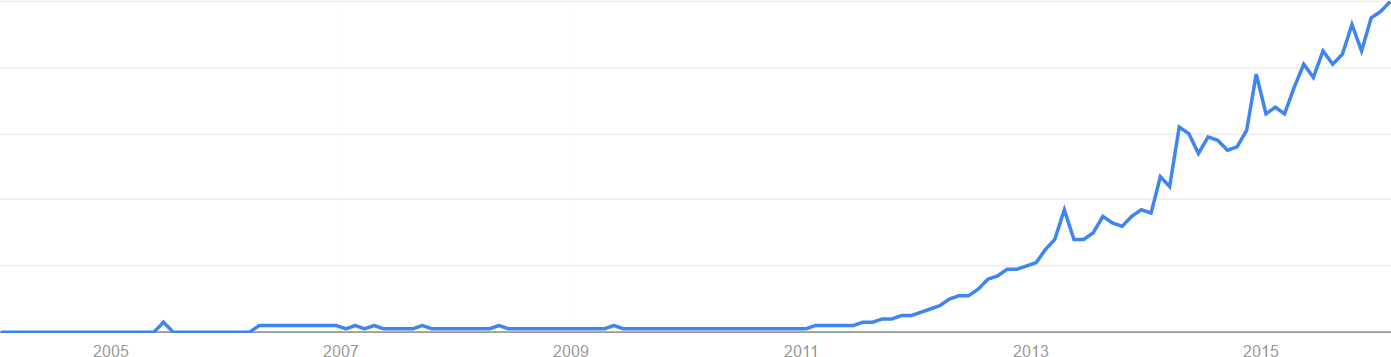
\includegraphics[width=0.9\columnwidth]{figures/google-trends}
  \caption{The popularity of ASMR searches has been rising steadily over the past four years. Data Source: Google Trends (\url{www.google.com/trends/}).}~\label{fig:google-trends}
\end{figure}

We explored whether the immersion, presence, and/or interactivity of a virtual reality system affects viewers' experience with media designed to evoke ASMR. This exploration was achieved through the use of standard VR equipment (described in more detail in Apparatus) and a custom-developed ASMR experience.

The ASMR experience that we created is one wherein the participant's avatar receives a virtual salon makeover. It consisted of a makeup artist, shown as a roughly animated 3D character, applying makeup to the participant's avatar. True to the format of ASMR videos, the artist moved around and spoke as they went about their tasks. The artist's speech was a pre-recorded mono track and positional audio was used to place it relative to the participant.

At certain points, the artist offered participants a selection of colours. A selection could be made by through head-tracking: by maintaining eye contact with the choice for a set time (see
Figure~\ref{fig:selection}). Choices made cosmetically affected the avatar displayed during the experience.

\begin{figure}[htb]
\centering
  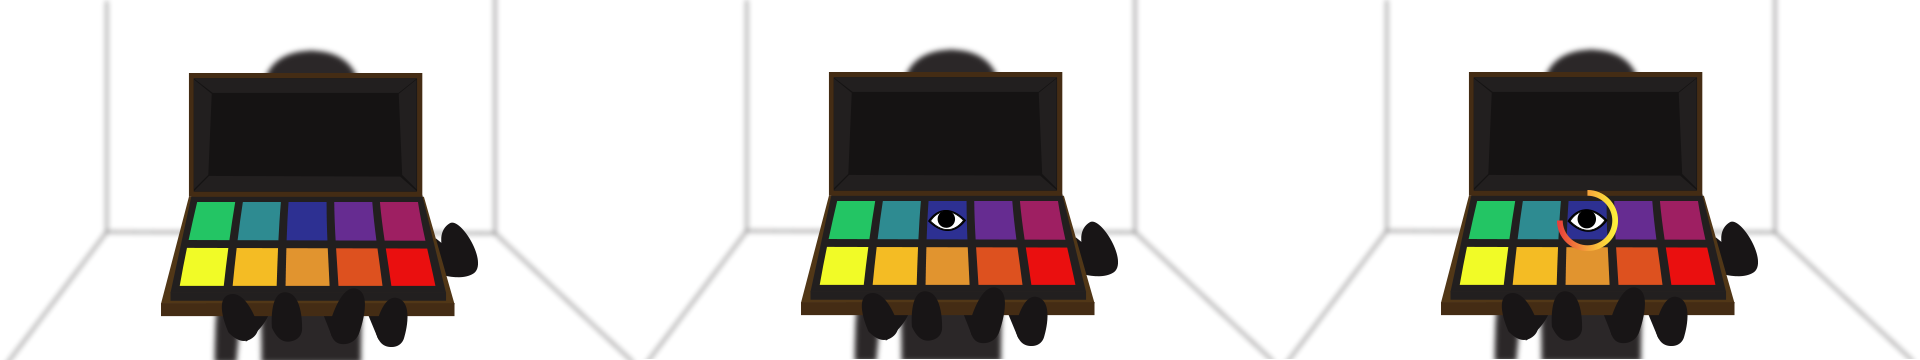
\includegraphics[width=0.9\columnwidth]{figures/selection}
  \caption{Mockup of the selection method which uses the center of the screen as a cursor position.}
  \label{fig:selection}
\end{figure}

\subsection{User Study}

To evaluate the experience, a comparative study was performed in which participants were exposed to two variations of the experience: one was the VR experience exactly as developed, and the other lacked visual stimuli and interaction in order to isolate audio, the component most closely associated with the YouTube ASMR format. The test used a within-subjects design, as individual differences would be a significant source of error for something as subjective as ASMR.

We hypothesized that the addition of visual stimuli and interaction with the system would further immerse the participant in the ASMR experience. As 98\% of individuals searching for ASMR videos have indicated that they do so for relaxation~\cite{barratt2015autonomous}, we evaluated the participant's sense of relaxation. This was measured through surveys and possible physiological indicators before, during and after the experience. We expected to observe higher satisfaction with the experience as a result of these factors than with passive audio alone.

\section{Related Work}

\subsection{Introduction to Autonomous Sensory Meridian Response}
Autonomous Sensory Meridian Response (ASMR, is the tingling sensation across the scalp and back of the neck, caused by specific audio and visual stimuli~\cite{barratt2015autonomous}. To experience ASMR, many users watch videos, often involving personal attention or grooming role-play \cite{andersen2015now,barratt2015autonomous} with a female host~\cite{andersen2015now} designed to elicit the phenomenon. Various types of stimuli can be used within a video to evoke the desired response~\cite{barratt2015autonomous}. When surveying those that experienced ASMR in order to learn which stimuli was triggering, it was found that whispering, personal attention, crisp sounds, and slow movements could cause the response. Whispering was the most common among participants, affecting 75\% \cite{barratt2015autonomous}. To increase the sensation, users may change their environment by dimming the lights or using headphones~\cite{begman2015}. For our project, we recorded similar audio stimuli to those listed above, and utilized high-fidelity headphones for the best experience. Since an HMD was used, dimming the lights was unnecessary.

Apart from eliciting a tingling sensation, ASMR is able to put users into a state similar to flow state, \inlinequote{the state of intense focus and diminished awareness of the passage of time that is often associated with optimal performance}~\cite{barratt2015autonomous}. During their research, Barratt and Davis observed that this state of concentration was improved with more ASMR triggers~\cite{barratt2015autonomous}. ASMR is valued for its calming effects \cite{barratt2015autonomous}; polls indicated that 98\% of users view ASMR videos for relaxation, and 70\% for stress relief~\cite{barratt2015autonomous}. Some believe in its effects enough to promote ASMR as a treatment for stress-related conditions such as anxiety~\cite{andersen2015now,begman2015}.

Unfortunately for those who use ASMR, these effects can be lost over long-time usage~\cite{andersen2015now}. In this situation, users often turn to more immersive experiences that use binaural sound and 3D microphones~\cite{andersen2015now}. It is believed that this adds to the experience's intimacy, heightening the response~\cite{andersen2015now}. 

\subsection{Virtual Reality Input Methods}
In a 2008 study, when comparing mouse and gaze pointing methods, participants perceived gaze as faster but less accurate than mouse pointing~\cite{mateo2008gaze}. Discomfort is a drawback of gaze pointing, especially if users must keep their heads still for a long time~\cite{mateo2008gaze}. We believe that the gaze method worked well for our project, as users were not be asked to complete tasks requiring accuracy or holding a position for a long time.

\subsection{The Effects of Virtual Reality}
Like real life environments, virtual environments can cause emotional reactions. During a 2007 experiment, it was found that when placed into a relaxation- or anxiety-inducing environment, participants showed signs of either relaxation or anxiety~\cite{riva2007affective}. It was also shown that a relaxing VR experience can increase feelings of quietness and happiness while reducing anger, sadness and anxiety~\cite{riva2007affective}. This suggests that virtual environments can be designed to evoke an emotional response from users~\cite{riva2007affective,wiederhold2006evaluation}. 

It was also found that the level of presence\footnote{\inlinequote{the \inlinequote{sense of being there} or the \inlinequote{feeling of being in a world that exists outside the self.}}~\cite{riva2007affective}} felt by participants was greater in relaxing and anxious environments than in neutral ones, and that the greatest feeling of presence was achieved in the relaxing environment~\cite{riva2007affective}. A previous review of virtual environments found that a participant's sense of presence is influenced by the attributes of the VR platform, the features of the environment itself, and the individuals characteristics~\cite{nash2000review}.

VR has also been seen as an alternative to therapy administration, which could help people in overcoming anxiety and stress-related conditions. It has been found in various studies that individuals enjoy VR therapy more than traditional therapy, leading to an increase in motivation to complete treatment~\cite{kizony2003adapting,morel2015advantages}. VR therapy also has the benefit of current equipment being affordable, allowing participants to engage in sessions in their own homes~\cite{morel2015advantages}. When researching the viability of VR therapy, a follow-up survey of those who suffered from anxiety found that there was no significant difference in the level of anxiety felt between participants of VR and traditional therapy~\cite{safir2011virtual}.

VR and ASMR have the shared capability of inducing relaxation and are both often used for therapeutic purposes. We combined these two relaxing mediums with the hope that users would be able to achieve a higher level of presence, and an increased perception of intimacy leading to an increase the effects of ASMR.

\subsection{Testing Methods}
To collect data on subjective topics, questionnaires are a useful tool. During Riva's experiment on the link between presence and emotions in multiple virtual environments, questionnaires were used to evaluate mood before and after the experience including Visual Analogue Scale (VAS), Positive and Negative Affect Schedule (PANAS), and State Trait Anxiety Inventory (STAI). The VAS required participants to indicate how they feel at a specific moment in time regarding their level of happiness, anger, surprise, disgust, anxiety and quietness. The PANAS uses a list of 20 adjectives that describe 10 positive and 10 negative emotions which can be viewed in Appendix~\ref{appendix:test_materials}. Participants must associate a magnitude on a scale of 1-5 for each emotion at a given moment. The STAI measures the level of anxiety participants feel on a scale of 0-3. The \inlinequote{State} version of this questionnaire asks participants how they feel at a given moment, while the \inlinequote{Trait} version asks for their general feelings. These questionnaires were provided to participants before and after testing to compare their baseline emotional state against the effects of the environment. Two additional questionnaires, the UCL Presence Questionnaire, and the Independent Television Company Sense of Presence Inventory (ITC-SOPI) were also given to participants after each stage in order to assess their presence. For the UCL Presence Questionnaire, please see Appendix~\ref{appendix:test_materials}.
The ITC-SOPI was used to measure different dimensions of presence, such as sense of physical space, engagement, ecological validity, and negative effects. The questionnaire is divided into two parts. The first consists of six items used to measure a participant's experience after the test has concluded, and the second consists of 38 items used to measure the participants experience during the test. Each is scored using a 5-point Likert scale~\cite{riva2007affective}.

Riva and her team also asked participants questions rated using a 10-point scale, while they were within the virtual environment. To measure their emotional status, participants were asked to what extent they felt sad, happy, anxious, and relaxed at any given moment. To measure presence, participants were asked if they felt as if they were in the virtual environment and whether that environment was a real place they were visiting. To view these questions, please see Appendix~\ref{appendix:test_materials}.
To reduce errors as a result of their within-subjects design, every participant was required to test each environment, with the sequence of environments being randomized~\cite{riva2007affective}.

For objective measurements on the emotional state of participants, physiological measures, such as heart-rate, can be taken. During a 2006 study on the effects of relaxation techniques and heart rate variability, it was found that guided relaxation decreased the participant's heart rate~\cite{sarang2006effects}. This shows a correlation between an individual's level of relaxation, which cannot directly be measured, and their heart rate.

To gather information on \inlinequote{the prevalence of particular features of ASMR, when and why individuals engage in ASMR, and the relation of ASMR to other known phenomenon}, Barratt and Davis collected information on a participant's viewing habits and various facets of their experience using a questionnaire~\cite{barratt2015autonomous}. Although this questionnaire is designed for use with those already familiar with ASMR, it could likely be used to assess the experiences of individuals new to the phenomenon. A version of the original questionnaire can be found in Appendix~\ref{appendix:test_materials}. 



\section{Methodology}

\subsection{Participants}
The test experiment was completed by 10 participants. The average age was 21.67 years old with a standard deviation of 1.41. Of the 10 participants, 6 were male, 3 were female, and 1 identifies as an other gender. All of the participants except for 1 had previous experience using VR. Three participants had previously experienced ASMR, listing their triggers as whispering and personal attention, whispering and crisp sounds, and crisp sounds respectively. None of the participants indicated that they watch ASMR videos in their daily life.

\begin{figure}[htb]
\centering
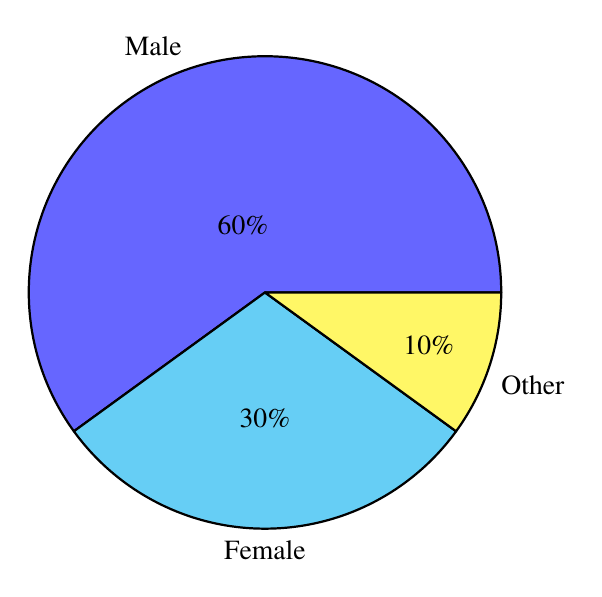
\begin{tikzpicture}
    \pie{60/Male, 30/Female, 10/Other}
\end{tikzpicture}
\caption{Gender of participants.}
\label{fig:gender}
\end{figure}

Of the 10 participants, one was excluded from the study as they indicated they had a history of heart problems in the family and suffered from a heart condition.

\subsection{Apparatus}
\begin{itemize}
\item{Oculus Rift DK2 (note: only the HMD's tracking is used; the external tracker which provides positional data is ignored for the purposes of this study)}
\item{S-Tengine2 game engine + \textit{Salon de Fr\'{e}Fr\'{e}} application
\begin{itemize}
\item{60 FPS}
\item{Approx. 30 ms latency}
\end{itemize}
}
\item{Grado SR80e headphones}
\item{Garmin FORERUNNER 410 + heart rate monitor attachment}
\item{Laptop
\begin{itemize}
\item{Windows 10 64-bit}
\item{16 GB RAM}
\item{Intel Core i7-3610QM CPU @ 2.30GHz 2.30 GHz}
\item{NVIDIA GeForce GTX 670M}
\end{itemize}
}
\end{itemize}
\subsubsection{Virtual Environment}
To enhance the relaxing effects of ASMR, the virtual environment used in the experiment was also designed to induce a similar relaxation response. This was done by creating an open space with high ceilings and large windows. Additionally, the environment used a calming pastel colour palette. 

\begin{figure}[htb]
\centering
  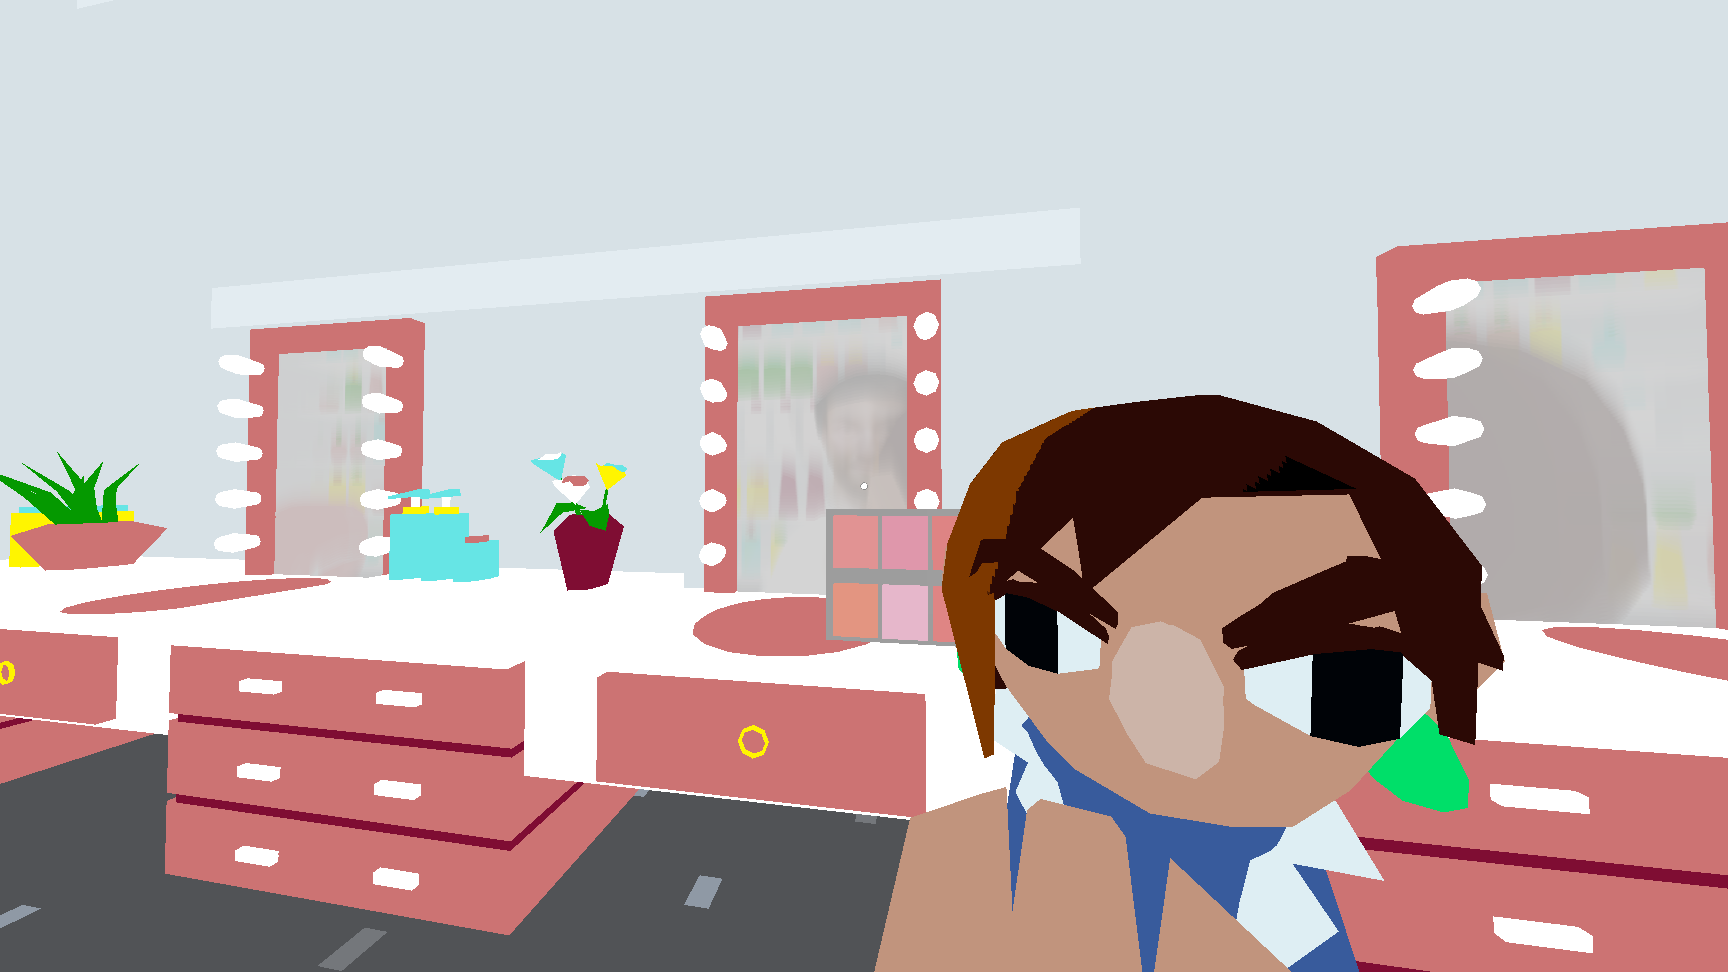
\includegraphics[width=0.9\columnwidth]{figures/game}
  \caption{Screenshot from \textit{Salon de Fr\'{e}Fr\'{e}}.}
  \label{fig:game}
\end{figure}

\subsection{Procedure}
A script (included in Appendix~\ref{appendix:script}) was read to the participants that informed them about the ASMR phenomenon, as well as the procedure they would have to follow during the test. They completed a pre-screening questionnaire to provide background information, and were asked to sign a consent form.

Participants were then asked to complete the two procedures outlined below. The order of these tests was alternated between participants to account for any confounding variables such as learning and comfort with the equipment.

\begin{figure}[htb]
\centering
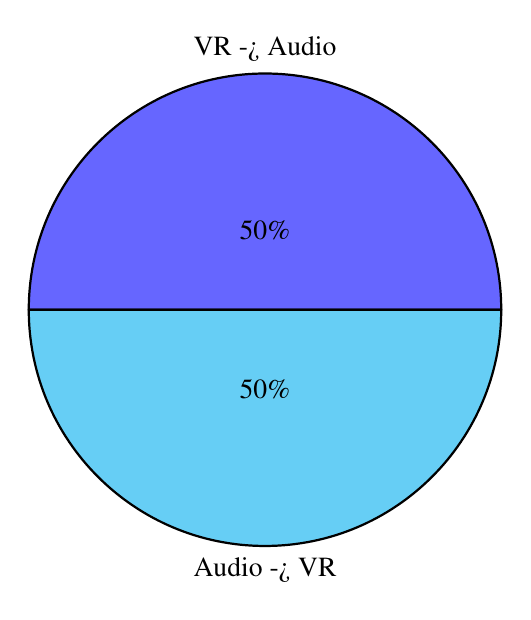
\begin{tikzpicture}
    \pie{50/VR -> Audio, 50/Audio -> VR}
\end{tikzpicture}
\caption{Testing order of participants.}
\label{fig:testing_order}
\end{figure}

The experiment took an average of 20 minutes to complete per participant.

\subsubsection{Virtual Reality + Audio}
\begin{enumerate}
\item{The participant is seated in an anechoic room and puts on the HMD and headphones with the aid of test moderators}
\item{The "Salon de Fr\'{e}Fr\'{e}" application is started by the test moderator}
\item{A makeup artist introduces herself}
\item{The artist asks participants to select a blush colour}
\item{Participants are presented with a palette and make a selection by looking at the option they want}
\item{The artist asks participants to select an eyeshadow colour}
\item{Participants are presented with a palette and make a selection by looking at the option they want}
\item{The artist asks participants to select an eyeliner colour}
\item{Participants are presented with a palette and make a selection by looking at the option they want}
\item{The artist asks participants to select a lipstick colour}
\item{Participants are presented with a palette and make a selection by looking at the option they want}
\item{Participants are informed that the makeup is complete and are told to look in the mirror}
\item{Participants remove the HMD and headphones}
\item{Participants complete a questionnaire}
\end{enumerate}

\subsubsection{Audio-only}
\begin{enumerate}
\item{The participant is seated in an anechoic room and puts on the HMD and headphones with the aid of test moderators}
\item{An audio file containing the entire experience is played}
\item{Participants remove the HMD and headphones}
\item{Participants complete a questionnaire}
\end{enumerate}






\section{Design}
This study is primarily concerned with an immersive VR experience's potential for affecting autonomous sensory meridian response. Two independent variables were identified and controlled during the study:
\begin{itemize}
\item{Positionally tracked stereo audio-visual vs. mono audio}
\item{Interactive head tracking vs. no head tracking (input/interactivity)}
\end{itemize}

Positionally tracked stereo audio-visuals were used with interactive head tracking in the immersive VR experience, while mono audio was used without any input or interactivity in the audio-only experience.

The results were measured as three dependent variables:

\begin{itemize}
\item{Subjective level of ASMR felt}
\item{Subjective level of relaxation felt}
\item{Change in heart rate}
\end{itemize}

Participants were asked to indicate whether they have experienced ASMR prior to the test, and if they have to list any triggers. They were then asked to indicate whether they experienced tingles following each test, and if they did, what they felt triggered these tingles. The level of relaxation felt was measured by asking participants for their mood prior to testing and asking for their mood following each test, if they felt as though their mood had changed. Change in heart rate was used as an objective, physiological way of measuring relaxation.

\subsection{Accommodations for Confounding Variables}
Before conducting testing, some confounding variables and ways to avoid them were identified. It is understood that ASMR is subjective, and as such data was taken from two trials that were completed by the same subject, rather than results between subjects. 

A heart rate sensor was used to measure relaxation. In order to understand if a participant's level of relaxation changed during the experiment, results were compared to a resting heart rate taken while in a relaxed state.

In addition to providing control over all of the independent variables, the apparatus introduces a number of unwanted variables. The HMD itself is a fairly large and bulky wearable display with many cables which can cause discomfort. In order to ensure that these variables did not affect the outcome of the study, the audio-only trial also required participants to wear the HMD despite the lack of visuals or head-tracking.

Similarly, the HMD and visuals used in the VR trial allowed for an interactive experience, and the user was able to actually select colours when asked by the makeup artist. During the audio-only trial, this form of interaction was impossible. In order to compensate for the discrepancy, additional questions were included in the makeup artist's script which cannot be answered in either the VR or audio-only trial; e.g. \inlinequote{What is your name?}

To minimise the possibility of breaks in presence as a result of outside noise or interactions, the trials were conducted in an environment which was as neutral as possible, an anechoic chamber, with only one observer present. This can be seen in Figure~\ref{fig:soundroom}. The observer only interacted with the participants prior to and after the trials, and remained silent as they were conducted.

\begin{figure}[htb]
\centering
  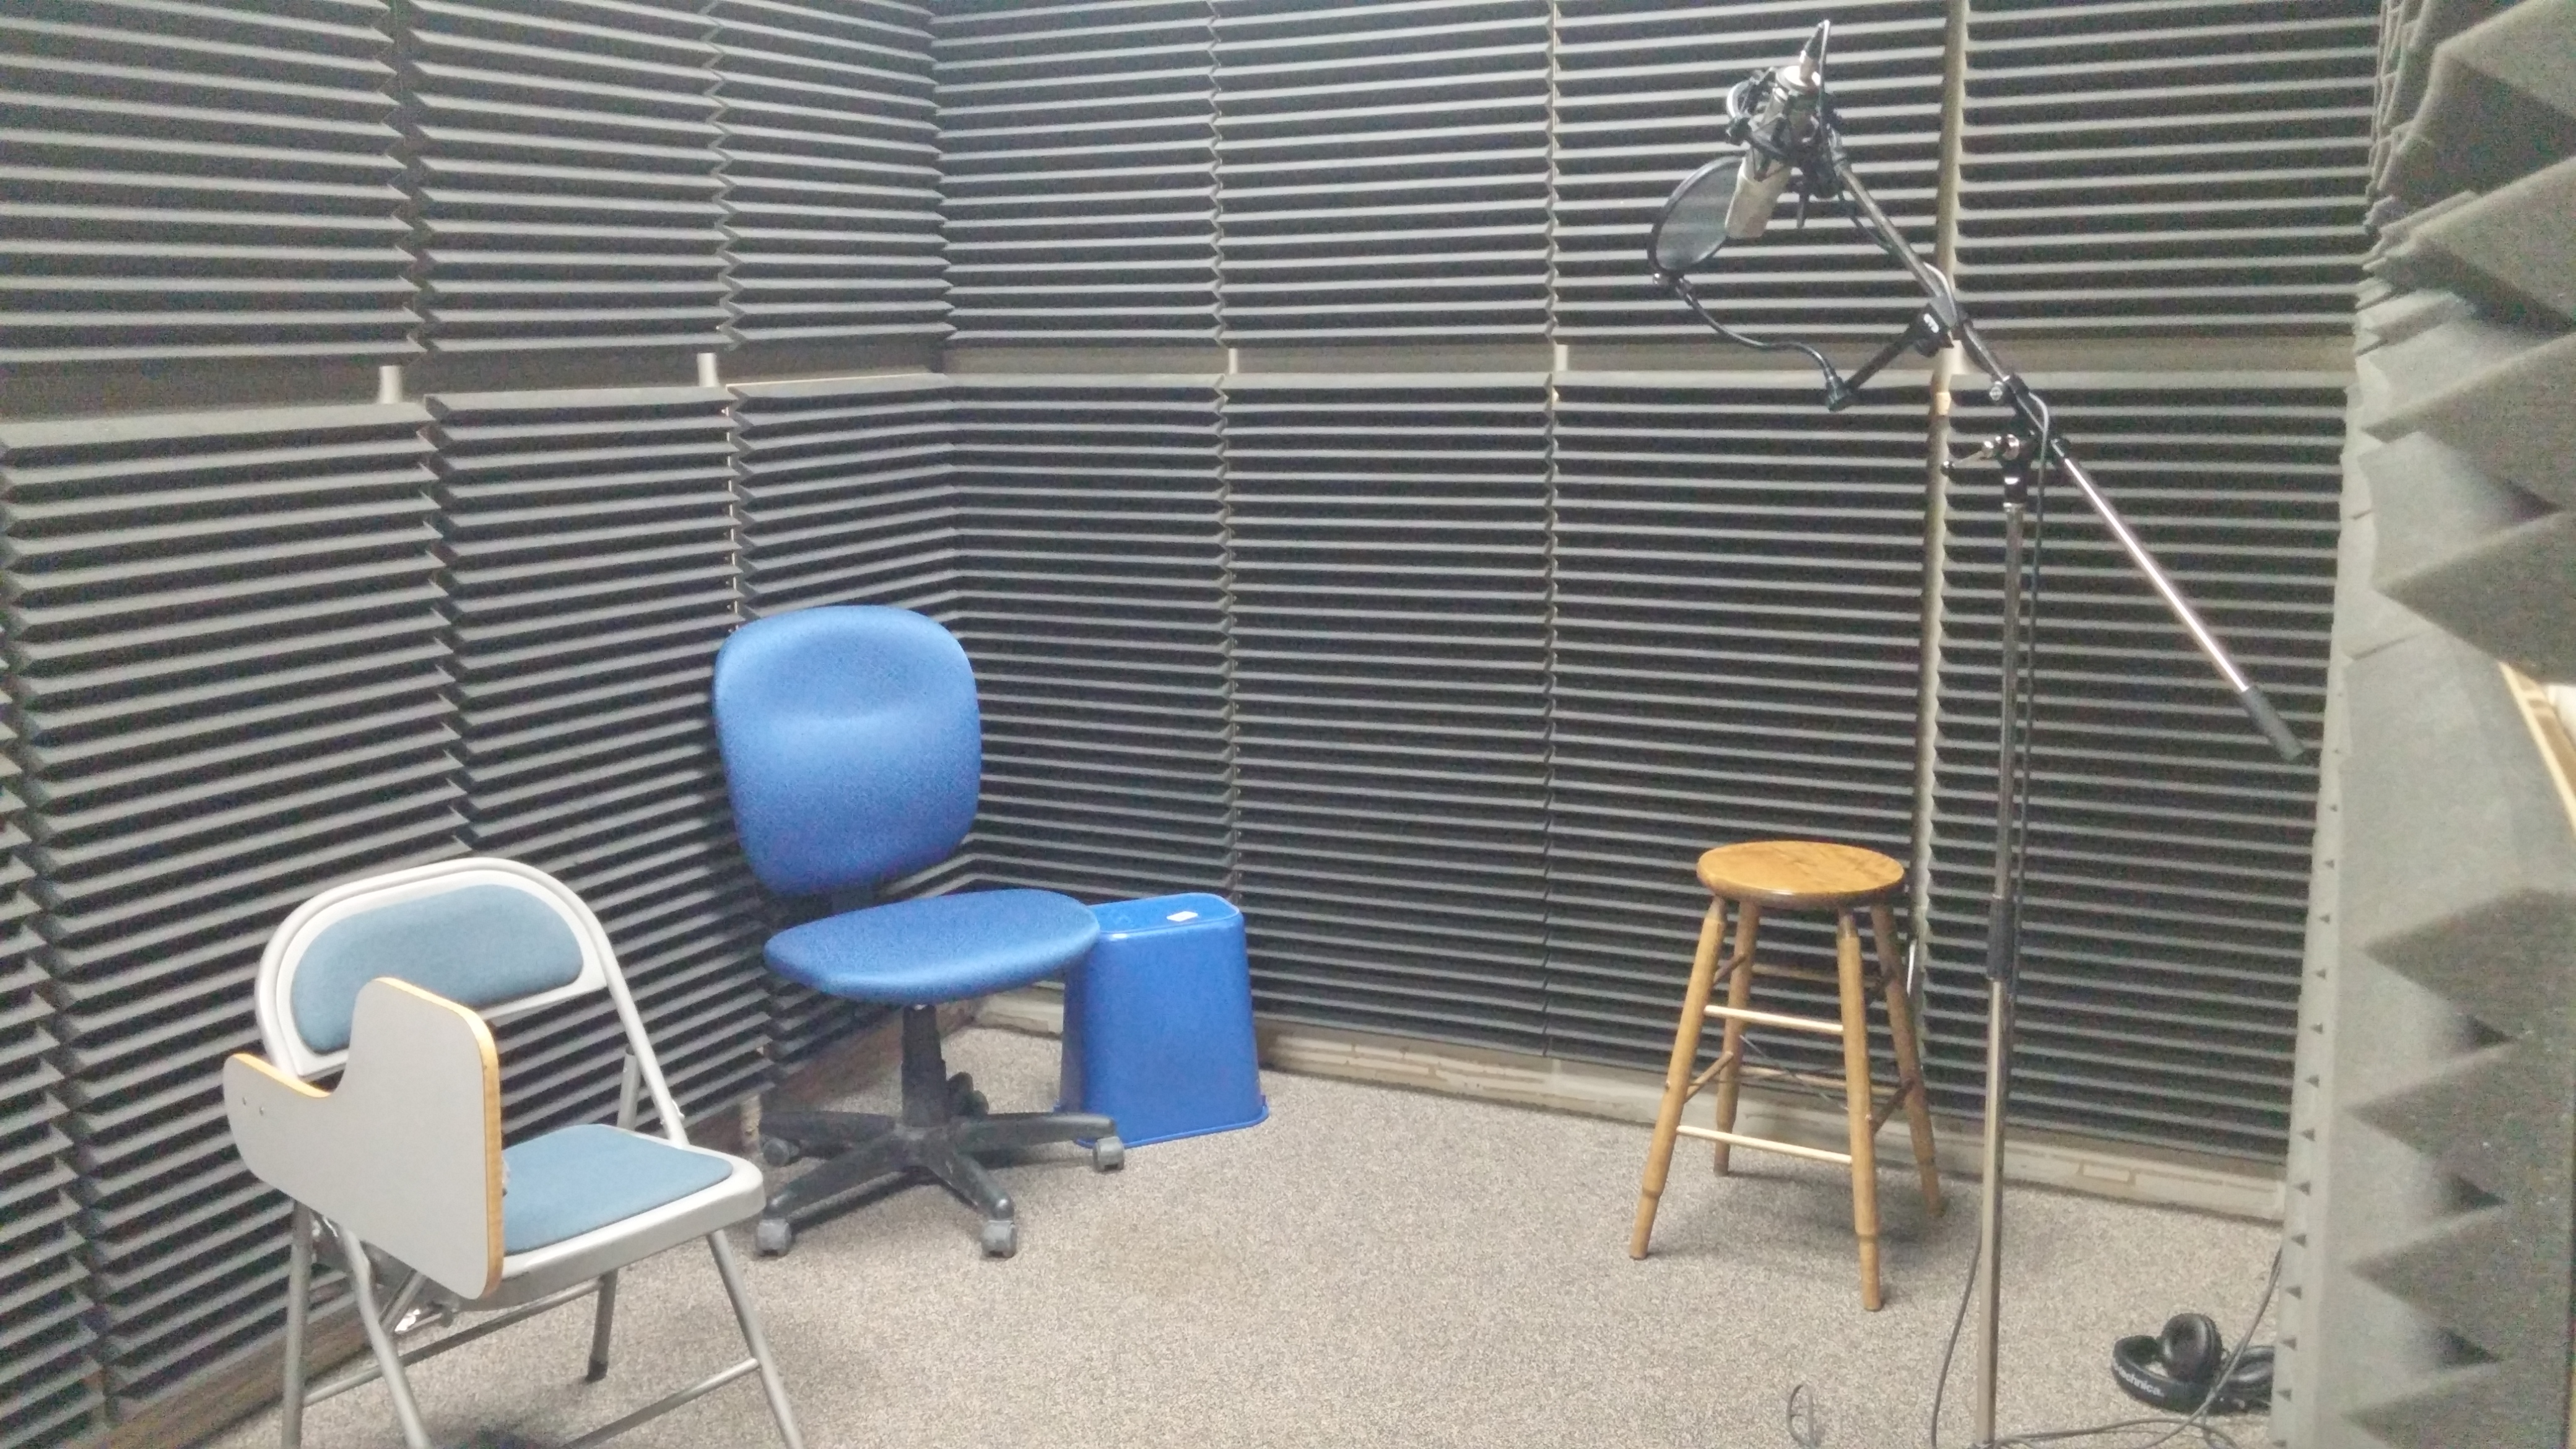
\includegraphics[width=0.9\columnwidth]{figures/soundroom}
  \caption{Location used for tesing.}
  \label{fig:soundroom}
\end{figure}




\section{Results \& Discussion}


\begin{table}[htb]
  \centering
  \begin{tabular}{l l}
    \toprule\\
    {\textit{Immersive VR}} & {\textit{Audio-only}}\\
    \midrule
    {Neutral to Neutral} & {Neutral to Relaxed} \\
    Neutral to Neutral & Relaxed to Neutral \\
    Happy to Neutral & Neutral to Neutral \\
    Happy to Relaxed & Relaxed to Neutral \\
    Neutral to Neutral & Neutral to Neutral \\
    Happy to Relaxed & Happy to Happy \\
    Neutral to Neutral & Neutral to Relaxed \\
    Neutral to Neutral & Neutral to Neutral \\
    Relaxed to Relaxed & Relaxed to Relaxed \\
     \bottomrule
  \end{tabular}
  \caption{Mood Change Indicated per Participant.}~\label{tab:mood_change}
\end{table}

Participant moods were compared between their baseline reading and their indicated mood following the first test, and their indicated mood following the first test and their indicated mood following the second test. These mood changes can be seen in Table~\ref{tab:mood_change}. 

It can be seen that two participants indicated a positive mood change, one indicated a negative mood change, and six participants indicated no perceivable change in mood for both the immersive VR experience and the audio-only experience. Although both tests were able to alter participant moods in a few cases, neither test proved better at affecting mood than the other.

\begin{figure}[htb]
\centering
\begin{tikzpicture}
\begin{axis}[
	x tick label style={
		/pgf/number format/1000 sep=},
	xlabel=Trial,
	ylabel=Experienced ASMR During Trial,
	enlarge x limits=0.9,
	legend style={at={(0.5,-0.2)},
		anchor=north,legend columns=-1},
	ybar,
	ymin=0,ymax=3,
	symbolic x coords={VR, Audio},
	xtick = data,
]

\addplot 
	coordinates {
	(VR,2)-+(1.65,2.65)
	(Audio,2)-+(1.65,2.65)
	};

\addplot 
	coordinates {
	(VR,1)-+(1.65,2.65)
	(Audio,2)-+(1.65,2.65)
	};

\legend{Experience with ASMR, No experience with ASMR}
\end{axis}
\end{tikzpicture}
\caption{ASMR in Participants.}
\label{fig:experienced_asmr}
\end{figure}

Two participants indicated that they had prior ASMR experience. As seen in Figure~\ref{fig:experienced_asmr}, both of these participants experienced ASMR during the immersive VR and audio-only tests, possibly indicating they are more predisposed to experiencing ASMR. 

Two participants that have never previously experienced ASMR experienced it during testing. Both participants indicated they felt tingles during the audio-only experience, and one participant indicated they also felt it during the immersive VR experience. Overall, four participants experienced ASMR during the audio-only experience, and three felt it during the immersive VR experience. There is a slight indication that the audio-only system is better at inducing ASMR in participants that the immersive VR system, however, the P value for this assertion was calculated as > 0.65 for a 2x2 contingency table, far outside the realm of statistically significant results.

\begin{table*}[htb]
  \centering
  \begin{tabular}{p{6cm} p{6cm} p{6cm}}
    \toprule\\
    {\textit{Previous ASMR triggers}} & {\textit{ASMR Triggers during Immersive VR}} & {\textit{ASMR Triggers during Audio-Only}}\\
    \midrule
    Whispering, Personal attention & Whispering & Whispering, Crisp sounds \\
    No known triggers & Crisp sounds & Whispering \\
    Whispering, Crisp sounds & Whispering, Positional audio (source behind participant) & Whispering, Illusion of positional audio (top of head)\\
    No known triggers & No ASMR experienced, Whispering, Crisp sounds\\
     \bottomrule
  \end{tabular}
  \caption{ASMR Triggers.}~\label{tab:triggers}
\end{table*}

As seen in Table~\ref{tab:triggers}, the two participants that had previously experienced ASMR indicated that their triggers were whispering and personal attention, and whispering and crisp sounds respectively. Whispering was a common trigger for participants, with all four participants indicating it caused their ASMR in the audio-only experience, and two participants listing it as a trigger during the immersive VR experience. Crisp sounds were indicated as a trigger in the audio-only experience by two participants, and by one participant in the immersive VR experience. One participant listed the location audio as being a trigger in both tests, even though the audio-only experience was presented in mono audio.

In addition to the questionnaires, objective heart-rate data was recorded for each participant during the testing. However, this data was excluded from the study as it was inconclusive. We believe further studies would benefit from the inclusion of heart-rate data, as there were extensive hardware issues throughout the trials which likely affected the results.

%discussion
Although the results of the two trials were fairly similar, the audio-only experience proved to be marginally more effective at evoking ASMR. Because of this, we rejected our original hypothesis; the data clearly shows that the addition of VR did not enhance the effects of ASMR, and in fact made it worse. This may be because when compared to the darkness of the audio-only trial, the immersive VR experience provided more stimulation and distracted participants from the audio, which was the most common trigger indicated in the surveys.

During the study, comments from a few participants revealed a minor bug with the software rendering, where the mirror displayed to users during the VR trial did not behave as expected. When users rotated their head around the y-axis, their virtual avatar's head rotated in the opposite direction. Although no one indicated this as having a significant effect on their overall experience, it had the potential to cause a break in presence and could bias their survey results in favour of the audio-only trial.

Unfortunately, the niche aspect of ASMR made finding people who actively seek out and enjoy ASMR difficult, and a larger sample which included more people with this trait could provide a more accurate data set.



%\begin{figure}[htb]
%\centering
%\begin{tikzpicture}
%\begin{axis}[
%	x tick label style={
%		/pgf/number format/1000 sep=},
%	xlabel=Question,
%	ylabel=Mean Score,
%	legend style={at={(0.5,-0.2)},
%		anchor=north,legend columns=-1},
%	ybar=4pt,
%	bar width=4pt,
%]
%\addplot+[error bars/.cd,y dir=both,y explicit]
%	coordinates {
%	(1930,1)+-(0.5,0.5)
%	(1940,2)
%	(1950,3)
%	(1960,4)
%	(1970,5)
%	};
%
%\addplot 
%	coordinates {
%	(1930,5)
%	(1940,4)
%	(1950,3)
%	(1960,2)
%	(1970,1)
%	};
%
%\addplot 
%	coordinates {
%	(1930,1)
%	(1940,2)
%	(1950,3)
%	(1960,4)
%	(1970,5)
%	};
%
%\legend{Baseline,VR,Audio}
%\end{axis}
%\end{tikzpicture}
%\caption{A bar graph!}
%\label{fig:bar_graph}
%\end{figure}

\section{Conclusion}
In conclusion virtual reality does not enhance the ASMR experience. Participants indicated that audio queues were the main trigger of tingles. The inclusion of interactive visual stimuli seems to have distracted users from the audio and has thus reduced the frequency of ASMR being triggered.


\subsection{Future Work}

A possible extension of this experience would be to have the test administrator brush the participant's face with actual makeup brushes in-sync with the virtual brushes. As we intended to primarily evaluate the visual and interactive elements, this idea was excluded from the study. We hypothesize that the haptic stimuli on its own could be capable of eliciting sensations similar to ASMR which would interfere with our own study~\cite{hall1897psychology}, and so we leave this for future works to consider.


%\section{Sample stuff}

%\begin{table}[htb]
  %\centering
 % \begin{tabular}{l r r r}
    % \toprule
 %   & & \multicolumn{2}{c}{\small{\textbf{Test Conditions}}} \\
 %   \cmidrule(r){3-4}
 %   {\small\textit{Name}}
 %   & {\small \textit{First}}
%      & {\small \textit{Second}}
 %   & {\small \textit{Final}} \\
  %  \midrule
  %  Marsden & 223.0 & 44 & 432,321 \\
  %  Nass & 22.2 & 16 & 234,333 \\
  %  Borriello & 22.9 & 11 & 93,123 \\
  %  Karat & 34.9 & 2200 & 103,322 \\
    % \bottomrule
%  \end{tabular}
%  \caption{Table captions should be placed below the table. We
%    recommend table lines be 1 point, 25\% black. Minimize use of
%    table grid lines.}~\label{tab:table1}
%\end{table}


%\begin{figure*}[htb]
%  \centering
%  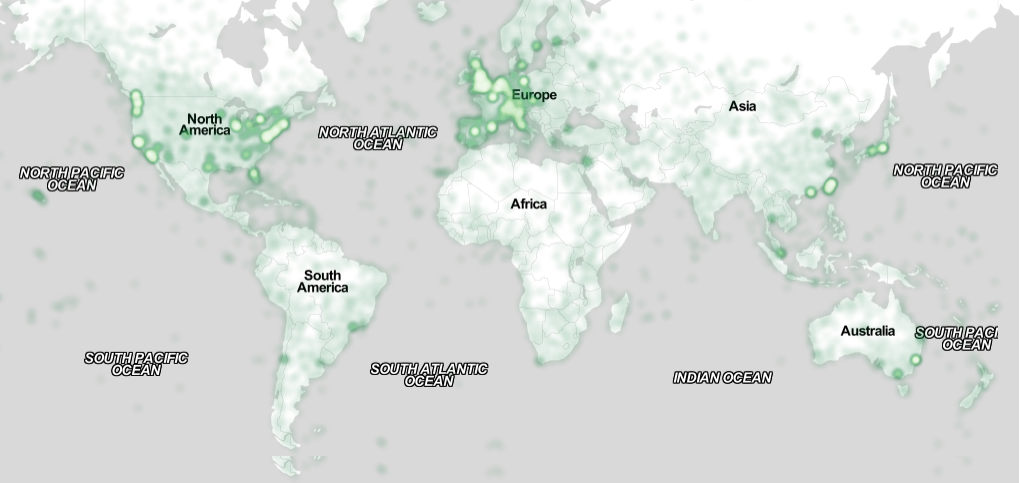
\includegraphics[width=1.75\columnwidth]{figures/map}
%  \caption{In this image, the map maximizes use of space. You can make
%    figures as wide as you need, up to a maximum of the full width of
%    both columns. Note that \LaTeX\ tends to render large figures on a
%    dedicated page. Image: \ccbynd~ayman on
%    Flickr.}~\label{fig:figure2}
%\end{figure*}

% Balancing columns in a ref list is a bit of a pain because you
% either use a hack like flushend or balance, or manually insert
% a column break.  http://www.tex.ac.uk/cgi-bin/texfaq2html?label=balance
% multicols doesn't work because we're already in two-column mode,
% and flushend isn't awesome, so I choose balance.  See this
% for more info: http://cs.brown.edu/system/software/latex/doc/balance.pdf
%
% Note that in a perfect world balance wants to be in the first
% column of the last page.
%
% If balance doesn't work for you, you can remove that and
% hard-code a column break into the bbl file right before you
% submit:
%
% http://stackoverflow.com/questions/2149854/how-to-manually-equalize-columns-
% in-an-ieee-paper-if-using-bibtex
%
% Or, just remove \balance and give up on balancing the last page.
%
\balance{}

% BALANCE COLUMNS
\balance{}

% REFERENCES FORMAT
% References must be the same font size as other body text.
\bibliographystyle{SIGCHI-Reference-Format}
\bibliography{sample}

\clearpage
\nobalance
\appendix


\section{Appendix A - Script}
\label{appendix:script}
\subsection{Introduction Script}
This study aims to determine whether the effects of ASMR can be triggered with more frequency or effectiveness through the addition of immersive VR. ASMR is the tingling sensation as a result of specific audio and/or visual stimuli. You will be asked to complete two trials of the provided virtual makeover experience, and answer a short questionnaire upon completion.

One trial will contain audio only and one will have both audio and visuals. Once the VR experience commences, please pretend that I am not here and do not talk to me. You may make verbal responses to the make-up artist if you so wish to.

\subsection{Immersive VR Script}
The makeup artist will ask you to make colour selections during the virtual makeover. To make a selection, look at the option you wish to select until the progress bar is complete. When the make-up artist asks you to look into the mirror, the makeover is complete and you may notify me so I can remove your equipment and you can fill out the survey.

\subsection{Audio only Script}
We will be asking you to wear the HMD even though there will be nothing playing on it. The audio track will be the same. You will be asked to complete a short survey when the experience ends.



\section{Appendix B - Questionnaires}
\label{appendix:questionnaire}
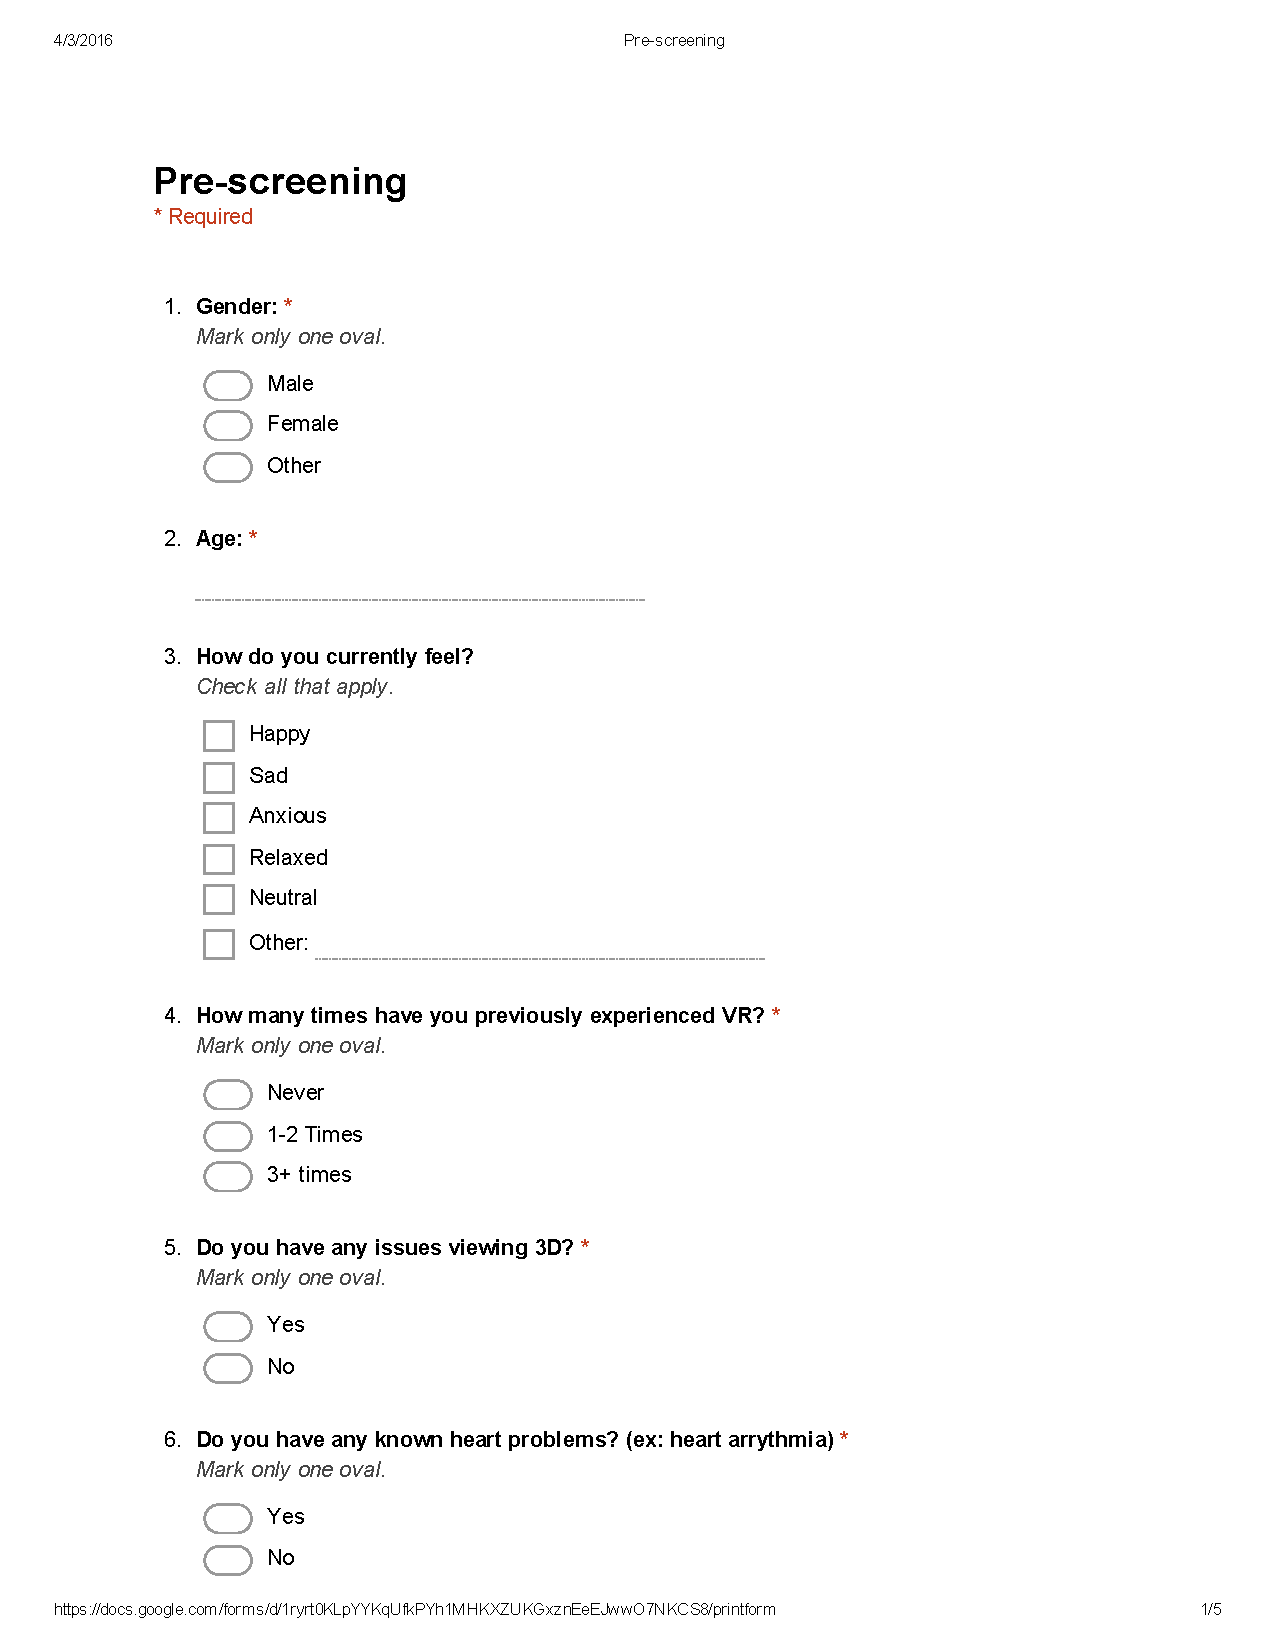
\includepdf[pages={1-}]{questionnaires/Google_Forms.pdf}





\section{Appendix C - Reference Test Materials}
\label{appendix:test_materials}
\subsection{UCL Presence Questionnaire}
For the UCL Presence Questionnaire, subjects were asked to answer using a 1-7 point Likert scale for the following questions:
\begin{enumerate}
	\item{\inlinequote{Rate your sense of being in the virtual environment.}}
	\item{\inlinequote{To what extent were there times during the experience when the virtual environment was reality for you?.}}
	\item{\inlinequote{When you think back to the experience, do you think of the virtual environment more as images that you saw or more	as somewhere that you visited?}}
	\end{enumerate}

\subsection{Affective Interactions Using Virtual Reality - Emotional Status and Presence Questionnaire}
To measure their emotional status, the following questions were asked:
\begin{enumerate}
	\item{\inlinequote{To what extent do you feel sad at this moment?}}
	\item{\inlinequote{To what extent do you feel happy at this	moment?}}
	\item{\inlinequote{To what extent do you feel anxious at this moment?}}
	\item{\inlinequote{To what extent do you feel relaxed at this moment?}}
\end{enumerate}

To measure presence, the following questions were asked:
\begin{enumerate}
	\item{\inlinequote{Do you feel you are here, in [the environment portrayed with virtual reality]?}}
	\item{\inlinequote{Do you feel this [virtual environment] is real, is it a place you are visiting?}}
\end{enumerate}

\subsection{Positive and Negative Affect Schedule}
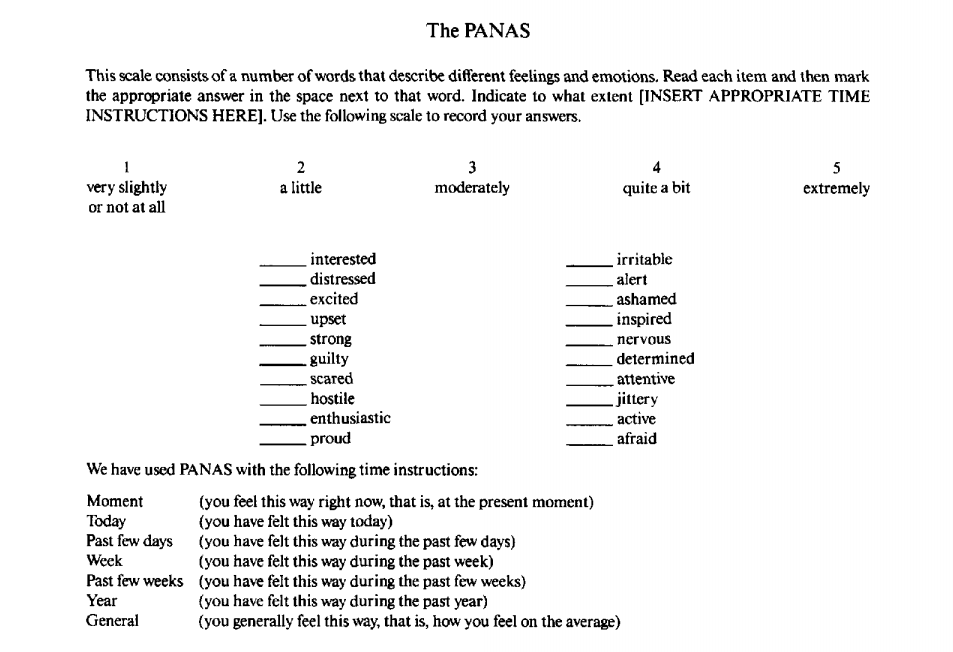
\includegraphics[width=0.5\textwidth]{questionnaires/ThePANAS.png}

\subsection{ASMR Questionnaire}
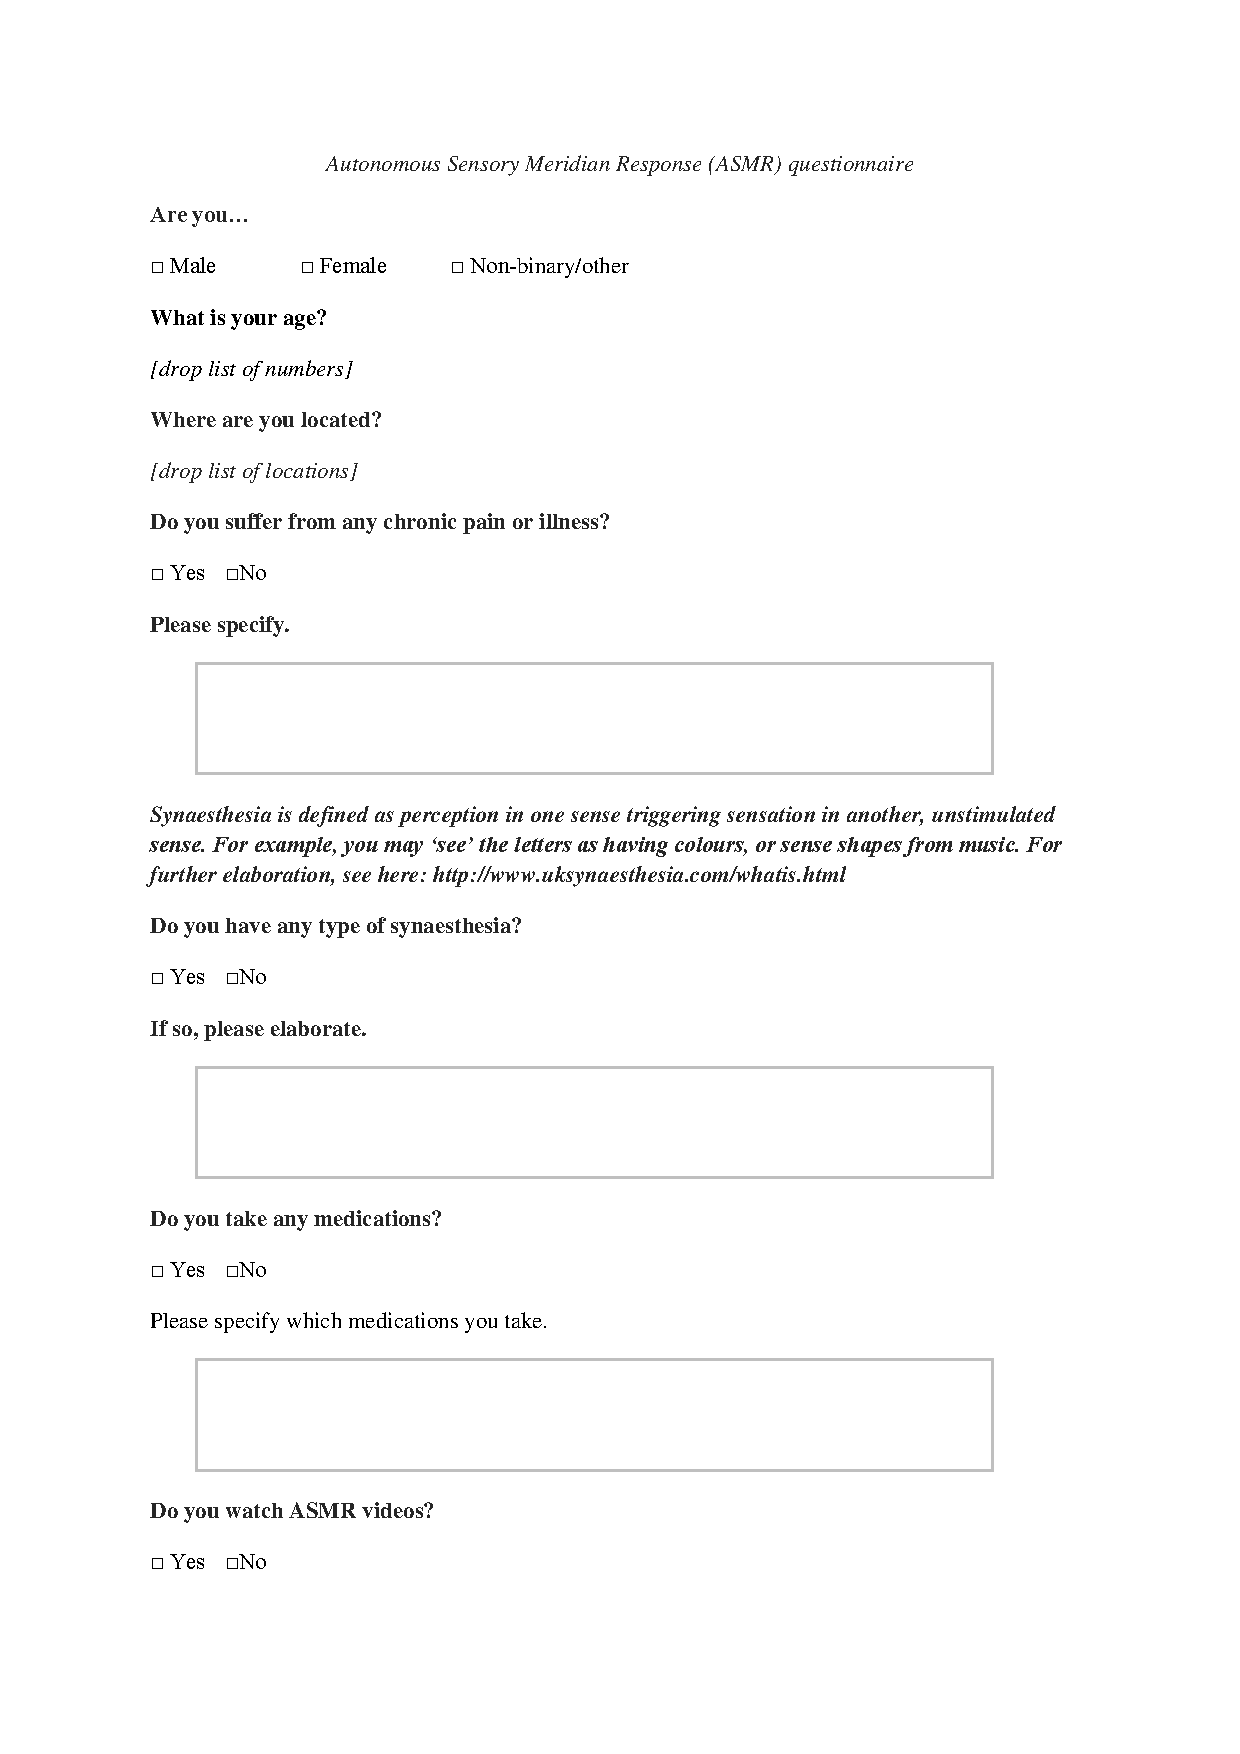
\includepdf[pages={1-}]{questionnaires/ASMR_Questions.pdf}



\end{document}

%%% Local Variables:
%%% mode: latex
%%% TeX-master: t
%%% End:
